% CAPITULO 1-------------------------------------------------------------------

\chapter{DESENVOLVIMENTO}
%\section{TAREFA 1}
%\label{sec:desenvolvimento}

A internet transformou o que antes era uma mensagem controlada e unilateral em um diálogo em tempo real, com milhões de pessoas, ao mesmo tempo.

Consequentemente, um plano de  comunicação  hoje não pode mais se basear em ações que não considerem o alcance e a velocidade com que as mensagens se espalham, principalmente pelo universo virtual.

Se hoje se conversa com milhões de pessoas ao mesmo tempo, assim deve ser a comunicação empresarial da nossa era, abrangente e em tempo real.

Essa necessidade tornou-se ainda mais imperativa após o surgimento das mídias online (incluindo as redes sociais, principalmente).

São milhões de menções no Twitter, likes no Facebook e feedbacks variados sendo publicados 24 horas por dia, 7 dias por semana.

Por conseguinte, o monitoramento dessas mídias, em tempo real, vem se tornando um diferencial competitivo indispensável para qualquer empresa ou marca que queira acompanhar seu posicionamento e sua reputação no mercado.

Seja para conhecer o comportamento do consumidor, para reagir a notícias negativas a tempo, para monitorar o mercado ou para vigiar os concorrentes, as mídias online podem ser consideradas, hoje, uma das fontes de dados mais valiosas a nosso dispor.

Em última instância, monitorá-las todas ainda ajuda a conectar marcas com seus clientes atuais e com os potenciais – aqueles que interagem com tópicos relacionados aos de interesse da sua empresa.

Sob a lógica dos negócios, portanto, não se pode ignorar o fenômeno das mídias online.

Pelo contrário, o seu acompanhamento em tempo real deve ser considerado prioridade máxima em qualquer empresa ou marca que queira ter reconhecimento, visibilidade e credibilidade no mercado. \cite{cortex}

Fazer o monitoramento integrado das mídias é um exemplo de como empresas podem combater \textit Fake \textit News, por isso ferramentas digitais ajudam na rápida disseminação de conteúdos verdadeiros logo que uma notícia falsa é detectada. Atenta a este cenário colaborativo empresa que trabalha com uma metodologia de modelagem de negócios, produtos e serviços inovadores, desenvolveu o MobNex, uma plataforma completa de mobilização colaborativa com o conceito de gamificação e colaboração, que integra um painel de controle da campanha com aplicativo e site. “Não é de hoje que notícias influenciam campanhas. Mas agora as fontes de informação são muito mais variadas e, às vezes, anônimas.

Pontua-se que ninguém está livre de protagonizar fake news que podem prejudicar suas campanhas. Esta é uma das vantagens estratégicas que plataformas como a Mobnex dá às campanhas: ajuda a combater as fake news, já que as pessoas que estão engajadas ajudam a disseminar conteúdos verdadeiros logo que uma notícia falsa é detectada.

Um dos diferenciais do MobNex é a possibilidade de ampliar a capacidade de mobilização pelo aplicativo, que possui estratégias de gamificação e conecta todos os envolvidos da campanha, atribuindo metas semanais de atuação, compartilhando informação em tempo real e valorizando os mobilizadores mais ativos. Campanhas altamente conectadas são mais ágeis e eficientes. Em tempos de grandes restrições, legais e orçamentárias, empoderar os mobilizadores é sair na frente. 

Os pesquisadores criaram um algoritmo, em códigos, com um sistema de detecção para atuar de forma automatizada. O caminho para a identificação da fake news é o seguinte: o método de inteligência computacional lê a notícia e extrai 21 características. A partir disso, uma etapa seguinte que verifica as características em três tipos: legítimo, falso ou irônico - chegando à análise final.

As 21 características são baseadas em informações textuais, como a utilização de pronomes e conjunções. Quatro dessas características foram definidas por eles: diversidade de classes gramaticais; frequência de personalidades reconhecidas, como o ex-presidente Obama; frequência de palavras fora de um domínio comum, como o da Política; frequência de aspas no texto. As outras 17 foram baseadas em pesquisas internacionais já realizadas.     

O caminho para a identificação é o seguinte: o método de inteligência computacional lê a notícia e extrai 21 características. A partir disso, uma etapa seguinte que verifica as características em três tipos: legítimo, falso ou irônico - chegando à análise final.

Quanto aos tipos de textos, os legítimos são os que contêm todas as informações verdadeiras; os falsos têm informações inventadas; já os irônicos misturam informações verdadeiras ou falsas com um tom de humor. O que já se percebe na verificação é que as notícias legítimas têm mais riqueza de vocabulário, qualidade de escrita. Nesses textos é possível perceber, por exemplo, a utilização de conjunção entre as frases, como o uso do "que", algo que não ocorre nas notícias falsas, que apresentam frases isoladas.

De acordo com o TSE, o bot Tira-dúvidas no WhatsApp traz diversos assuntos de interesse do eleitor, que vão desde informações sobre dia, horário e local de votação, até dicas para mesários. Por meio de uma conversa com o chatbot, é possível acessar os principais links de serviço, baixar o aplicativo e-Título e conferir as principais dicas para eleitores e mesários, além de justificar a ausência às urnas.
O assistente virtual oferece ainda um serviço voltado exclusivamente ao esclarecimento de notícias falsas envolvendo o processo eleitoral brasileiro: o “Fato ou Boato? ”. Ao selecionar o tópico, o usuário pode acessar alguns conteúdos desmentidos por agências de checagem de fatos e desmistificar os principais boatos sobre a urna eletrônica.

\section{Middleware} % (fold)
\label{sec:middleware}

Além da criação do chatbot, a parceria entre o TSE e WhatsApp prevê a criação de uma página para que os usuários possam denunciar contas suspeitas de realizar disparos em massa – uma das condutas proibidas pela lei eleitoral e também pelos Termos de Serviço do aplicativo. Se você viu ou desconfia de algum desses grupos no seu WhatsApp, pode fazer sua denúncia preenchendo um formulário. O middleware é o software que se encontra entre o sistema operacional e os aplicativos nele executados. Funcionando de forma essencial como uma camada oculta de tradução, o middleware permite a comunicação e o gerenciamento de dados para aplicativos distribuídos.

Muitas vezes, o middleware é chamado de “encanamento”, uma vez que ele conecta dois aplicativos para que os dados e bancos de dados possam ser facilmente transportados através do “cano”. O uso do middleware permite que os usuários executem solicitações como enviar formulários em um navegador da Web ou permitir que o servidor Web apresente páginas dinâmicas da web com base no perfil de um usuário.

Exemplos comuns de middleware incluem middleware de banco de dados, middleware de servidor de aplicativos, middleware orientado a mensagens, middleware de web e monitores de processamento de transações. Normalmente, cada programa oferece serviços de sistemas de mensagens para que diversos aplicativos possam se comunicar utilizando estruturas de mensagens como protocolo SOAP, serviços Web, REST (representational state transfer) e JSON (JavaScript Object Notation). 

Embora todos os tipos de middleware executem funções de comunicação, o tipo que uma empresa escolherá depende de qual serviço está sendo utilizado e qual tipo de informação deve ser comunicado. Isso pode incluir autenticação de segurança, gerenciamento de transações, consultas de mensagens, servidores de aplicativos, servidores da web e diretórios. O middleware também pode ser utilizado para processamento distribuído com ações que ocorrem em tempo real em vez de envio e recebimento repetitivo de dados.

\section{Media Queries}
\label{sec:mediaqueries}

Media queries é uma técnica de consulta de mídia que atribui diferentes estilos CSS para diferentes resoluções de tela possibilitando assim fornecer um visual diferente a cada resolução detectada.

As Media queries definem condições para utilização de estilos CSS. Se o dispositivo de acesso do usuário se adequar as condições se aplicam os estilos.

Os conceitos de breakpoints podem enfim serem aplicados agora com as Media queries pois seus valores são utilizados na sintaxe para definir a partir de qual ponto se aplicará os estilos CSS. \cite{responsivo}

\begin{figure}[!htb]
    \centering
    \sbox0{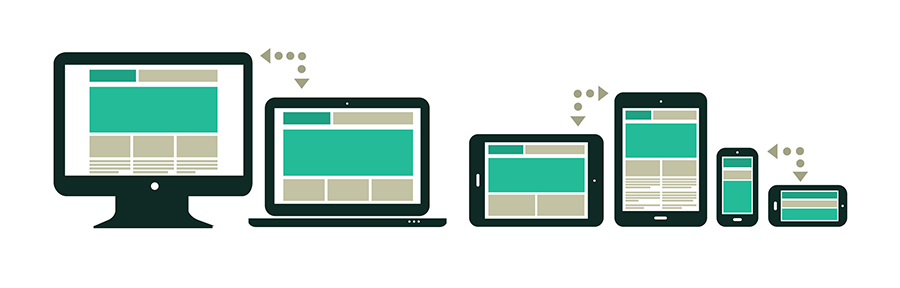
\includegraphics[width=0.5\textwidth]{./dados/figuras/figura1}}  % measure width
    \begin{minipage}{\wd0}
    \usebox0
        \caption{Media Query - adaptado pelo autor}
    \end{minipage}
\end{figure}

\section{Desenvolvimento Híbrido}
\label{sec:desenvolvimentohibrido}

Hoje o desenvolvimento mobile segue basicamente 2 caminhos para construir um APP: Nativo ou Híbrido. Qual a diferença entre eles e qual o melhor cenário para uso de cada um ?
 
Desenvolvimento Nativo é quando o usamos o código puro e específico da plataforma que pretendemos entregar nosso app, por exemplo, Android ou IOS. No caso do Android usamos Java e para IOS as linguagens podem ser Objective-C ou ou Swift (a mais recente).
 
Desenvolvimento híbrido é a mistura de tecnologias Web, como HTML5, Javascript e CSS,em conjunto com algum framework que tenha acesso às funções nativas do aparelho, como sensores, acelerômetro e câmera, por exemplo. Esta modalidade tem ganhado muito espaço pois desenvolvedores web podem facilmente migrar para o desenvolvimento de apps híbridos, visto que a curva de aprendizado é bem menor do que aprender Java e a API do Android, por exemplo.

Apps Nativos
App Nativo é recomendado para casos específicos, onde a performance é imprescindível, principalmente em apps que vão usar muitos gráficos, como jogos. Performance ainda é o calcanhar de Aquiles dos apps híbridos, embora os frameworks tenham evoluído muito nessa questão de uns tempos para cá. Desenvolver um App nativo custa mais caro, pois demanda mais tempo e precisa de um programador específico naquela plataforma.

Apps Híbridos
Já o desenvolvimento híbrido é recomendado para não demandem performance robusta e funções avançadas. A maior vantagem, além do custo, é a portabilidade do código, ou seja, com pequenos ajustes o mesmo aplicativo pode ser lançado paras as diversas plataformas, como Android, IOS, Firefox OS, etc. \cite{hibrido}

%O HTML foi criado para ser portável, ou seja, ele deve ser lido e interpretado por qualquer tipo de dispositivo. Cada dispositivo exibe HTML de uma determinada maneira. Logo, a forma com que você formata o layout precisa ser diferente para cada dispositivo. Por exemplo, se alguém visita um site por um desktop, a experiência será totalmente diferente caso você visite o mesmo site por um dispositivo móvel. São dispositivos diferentes, com formas totalmente diferentes de navegação e uso.
%O desenvolvimento de apps multiplataforma (ou híbridos) também ganhou impulso e certamente o crédito é aos frameworks. Pois, desempenham um papel crucial na conversão de um app Android em um app para iOS e vice-versa.

\section{Frameworks}
\label{sec:frameworks}

Segundo a Wikipédia, um framework é uma abstração que une códigos comuns entre vários projetos de software provendo uma funcionalidade genérica. Um framework pode atingir uma funcionalidade específica, por configuração, durante a programação de uma aplicação. Ao contrário das bibliotecas, é o framework quem dita o fluxo de controle da aplicação, chamado de Inversão de Controle. \cite{framew}

O Ionic é um framework amplamente utilizado para o desenvolvimento de aplicativos. O que é mais interessante notar é que ele é gratuito. Geralmente, é um framework do lado do cliente que ajuda na criação de aplicativos nativos com uma combinação de HTML, CSS3 e JavaScript.
A framework Ionic também suporta os dispositivos mais recentes e prepara um terreno robusto para os aplicativos antes do seu lançamento no mercado.

O elemento do HTML5 também ajuda na criação de aplicativos híbridos. E não há dúvida de que ele é considerado um dos melhores frameworks para o desenvolvimento dos Progressive Web Apps.
React Native é um dos outros frameworks multiplataforma populares que foi lançado pelo rei das mídias sociais, o Facebook. Embora a sua criação tenha sido feita há pouco tempo, em 2013, tornou-se uma das opções preferidas para os desenvolvedores de aplicativos móveis.

O React Native é basicamente um framework de código aberto que oferece amplo suporte aos IDEs e às outras ferramentas de desenvolvimento de aplicativos. Supõe-se que seja um dos melhores frameworks JavaScript para criar aplicativos nativos para as plataformas Android e iOS. Há a opção de escolher o React, para web, e o React Native para o desenvolvimento de aplicativos móveis.
